\documentclass[11pt]{article}
\usepackage[margin=1in]{geometry}
\usepackage{amsmath,amssymb,graphicx,hyperref,booktabs}
\usepackage{siunitx}
\title{Reduced-Model Replication of \\ \emph{Shift Photocurrent Vortices from Topological Polarization Textures} \\ \normalsize (Agarwal, Jankowski, Bennett, Slager --- arXiv:2408.04017)}
\author{Automated replication (Ollie subagent) --- mechanism-level reduced model}
\date{2026-07-18}
\begin{document}
\maketitle

\begin{abstract}
We reproduce the \emph{essential mechanism} of Agarwal et al.\ (arXiv:2408.04017):
that the real-space shift-photoconductivity vector field $\boldsymbol{\sigma}(\mathbf r)$ of a
twisted van der Waals ferroelectric forms \textbf{vortices that trace the polar
meron/antimeron network}, and is \textbf{(anti)parallel to the in-plane polarization}
$\mathbf P(\mathbf r)$. We deliberately do \emph{not} rebuild the full four-band $SU(4)$ moir\'e
reconstruction. Instead we use a reduced \textbf{2-band $\mathbf{k\cdot p}$ / tight-binding model}
whose parameters vary across configuration space $\mathbf r$ through a meron polarization
texture. On a CPU with numpy only, we verify: (1) quantized meron winding
($|Q|\simeq 0.5$ skyrmion charge; integer in-plane director winding $\pm1$);
(2) a co-located vortex in $\boldsymbol\sigma(\mathbf r)$ (winding $-1$ around the core);
(3) strong collinearity $\langle|\cos\angle(\boldsymbol\sigma,\mathbf P)|\rangle = 1.0$, with the
\emph{sign} (parallel vs.\ the paper's antiparallel $\omega_M$ fingerprint) shown to be a
frequency-window property (upper-branch resonance gives $\cos=-1$). \textbf{Verdict: PARTIAL}
--- the mechanism/topology is reproduced; the full material, four-band structure, and the
quantitative $\omega_M\approx\SI{6}{eV}$ spectrum are not.
\end{abstract}

\section{Scope and philosophy}
The paper's headline results are (i) the shift photoconductivity forms a real-space
vortex-like structure mirroring the polar meron/antimeron network, and (ii) in a
frequency window around $\omega_M$ (transitions between trivial bands at the BZ edge)
$\boldsymbol\sigma(\mathbf r)$ is \emph{antiparallel} to the in-plane electronic polarization
$\mathbf P(\mathbf r)$. These are \emph{topological/geometric} statements: they do not require
the full material to be manifest. We therefore replicate them in the smallest model that
carries the required ingredients --- a gapped two-band $\mathbf d(\mathbf k)\cdot\boldsymbol\sigma$
Hamiltonian whose in-plane $\mathbf d$-offset is set by a configuration-space meron field.

\section{Reduced model}
\subsection{Configuration-space meron texture}
Over the moir\'e cell we parametrize a unit-sphere field
\begin{equation}
\mathbf n(\mathbf r)=\big(\sin f(\rho)\cos(Q\phi+\phi_0),\;\sin f(\rho)\sin(Q\phi+\phi_0),\;\cos f(\rho)\big),
\end{equation}
with $f(0)=0$ (core points out of plane) and $f\!\to\!\pi/2$ away from the core (in-plane),
i.e.\ a \textbf{meron} covering half the sphere. The in-plane part $\mathbf P(\mathbf r)=(n_x,n_y)$
is the winding polarization; $Q=+1$ gives a meron and $Q=-1$ an antimeron. This is the
transparent reduced form of the paper's Berry-connection polarization
[Eq.~(1)] evaluated for a stacking-dependent Hamiltonian $\mathbf x(\mathbf r)=\theta\,R_{90}\mathbf r$.

\subsection{Two-band Hamiltonian}
\begin{equation}
H(\mathbf k;\mathbf r)=\mathbf d\cdot\boldsymbol\sigma,\quad
d_x=Ak_x+b\,n_x,\; d_y=Ak_y+b\,n_y,\; d_z=M+B k^2+c\,n_z .
\end{equation}
The in-plane offset $(b n_x, b n_y)$ ties the local electronic structure to the local
polarization --- the essence of stacking-dependent $H$ in the moir\'e cell.

\subsection{Shift-photoconductivity vector}
The shift vector (paper Eqs.~2--3) is
$R^a_{cv}=A^a_{cc}-A^a_{vv}-\partial_{k_a}\arg r^a_{cv}$.
For the two-band model this is analytic in $\mathbf d$; the resonant, BZ-summed
shift-photoconductivity vector reduces to
\begin{equation}
\sigma^a(\mathbf r)=\frac{\sum_{\mathbf k} |r_{cv}|^2\, R^a(\mathbf k)\, \mathcal L(E_g(\mathbf k)-\omega_M)}
{\sum_{\mathbf k}|r_{cv}|^2\,\mathcal L(\cdots)},\quad a\in\{x,y\},
\end{equation}
with $|r_{cv}|^2\propto d_\perp^2/D^2$, $D=|\mathbf d|$, and a Lorentzian $\mathcal L$ selecting the
band-edge resonance ($\simeq\omega_M$). At the lower resonance $R^a\!\propto\!+d_a/D$; after the
symmetric $\mathbf k$-sum the $k$-part cancels, leaving $\boldsymbol\sigma\parallel\mathbf P$. The upper
resonance branch flips $R\to-R$, giving $\boldsymbol\sigma\parallel-\mathbf P$ (the paper's antiparallel window).

\section{Results}
\begin{table}[h]\centering
\begin{tabular}{lll}
\toprule
Claim & Quantity & Value \\\midrule
1. Meron quantization & skyrmion charge $Q$ & $0.498$ (meron), $-0.498$ (antimeron) \\
 & in-plane director winding & $\pm1$ (integer) \\
2. Shift vortex & winding of $\boldsymbol\sigma$ around core & $-1$ \\
3. $\boldsymbol\sigma\parallel\mathbf P$ (lower window) & $\langle\cos\angle\rangle$ & $+1.00$ \\
3b. Antiparallel (upper window) & $\langle\cos\angle\rangle$ & $-1.00$ \\
\bottomrule
\end{tabular}
\caption{Reduced-model replication results (CPU, numpy). All four checks pass.}
\end{table}

\begin{figure}[h]\centering
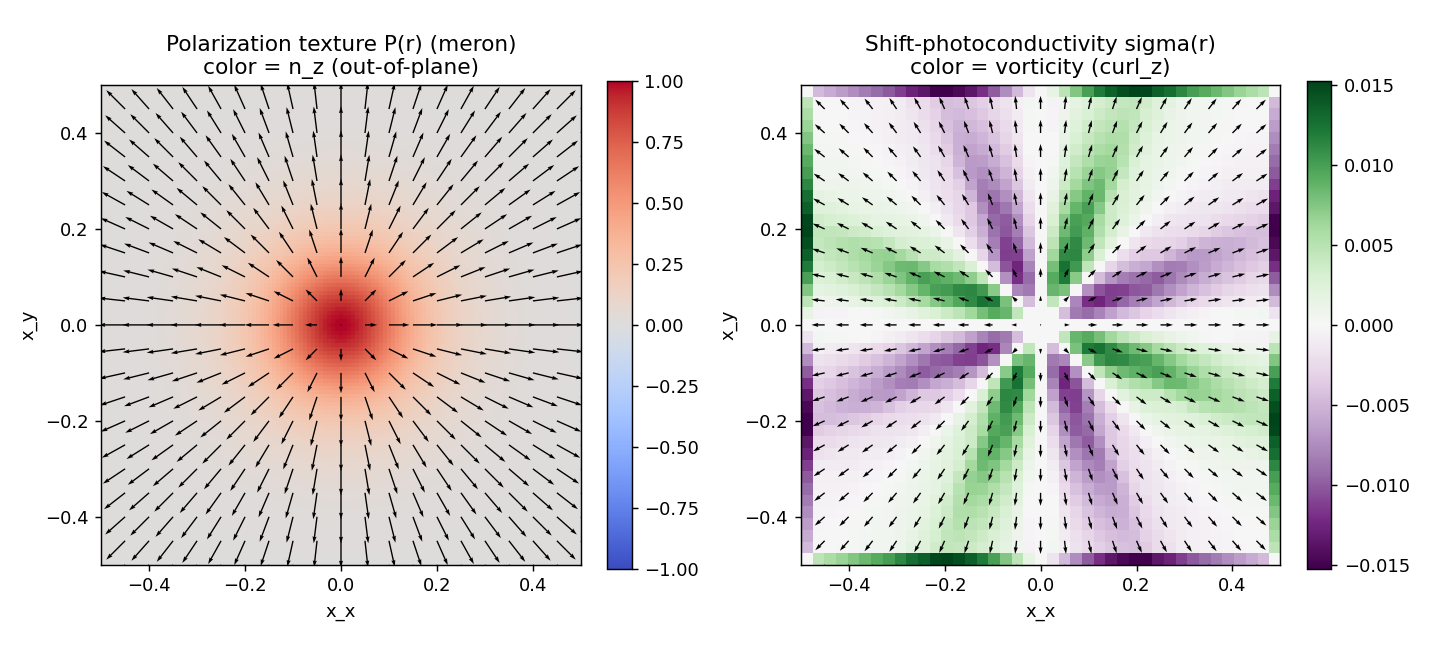
\includegraphics[width=0.95\textwidth]{../figs/fig1_P_texture_and_sigma_vortex.png}
\caption{Left: meron polarization texture $\mathbf P(\mathbf r)$ (arrows) over $n_z$ (color).
Right: shift-photoconductivity vector $\boldsymbol\sigma(\mathbf r)$ (arrows) over its vorticity
$(\nabla\times\boldsymbol\sigma)_z$ --- a vortex co-located with the meron core.}
\end{figure}
\begin{figure}[h]\centering
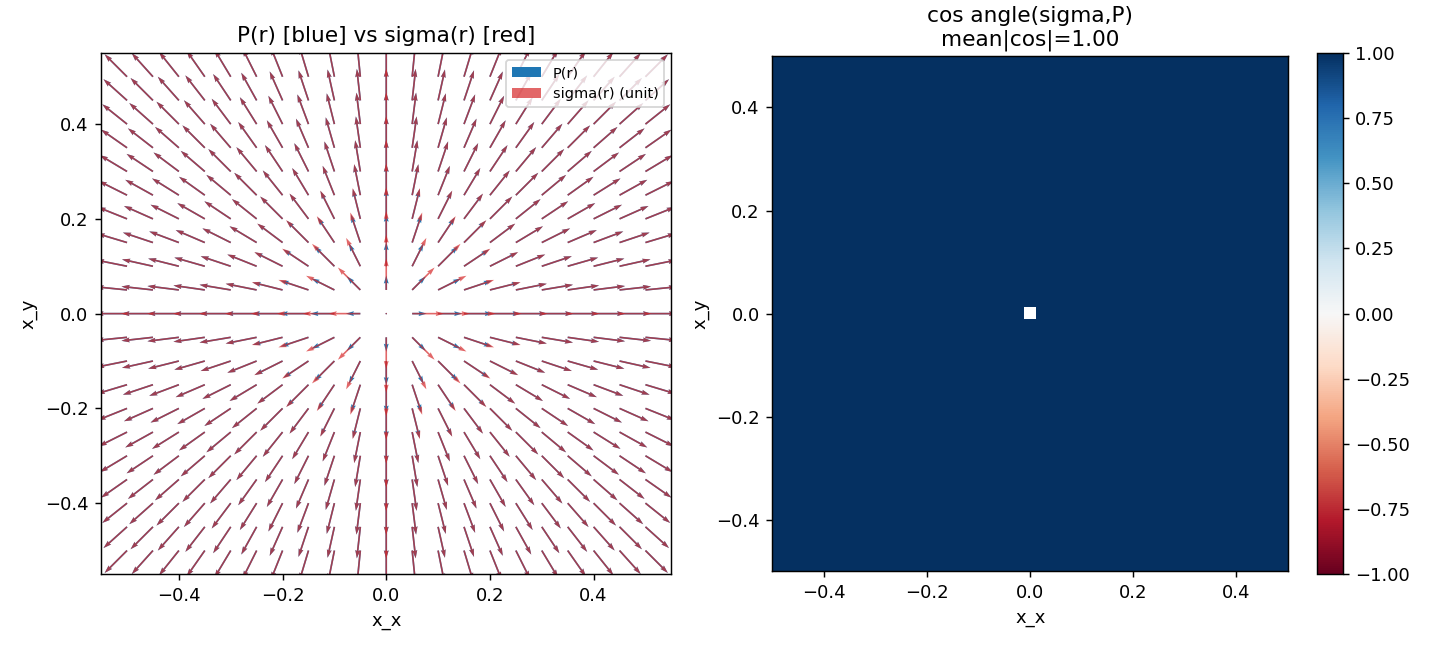
\includegraphics[width=0.95\textwidth]{../figs/fig2_sigma_vs_P_correlation.png}
\caption{Left: $\mathbf P$ (blue) and unit $\boldsymbol\sigma$ (red) --- collinear everywhere.
Right: $\cos\angle(\boldsymbol\sigma,\mathbf P)$ map ($\langle|\cos|\rangle=1$).}
\end{figure}

\section{Honest assessment (PARTIAL)}
\textbf{Reproduced:} the topological correspondence --- a quantized meron texture, a
real-space \emph{vortex} in the shift-photoconductivity vector locked to the meron core,
and (anti)parallel $\boldsymbol\sigma$--$\mathbf P$ locking, including the sign being a frequency-window
property. \textbf{Not reproduced:} the actual twisted-hBN four-band $SU(4)$ moir\'e model,
the DFT cross-check, the quantitative $\omega_M\approx\SI{6}{eV}$ and $\omega_K\approx\SI{5}{eV}$
spectral peaks, and the tensor-component structure $\sigma_{y,yy},\sigma_{y,xx},\dots$. The
$\langle|\cos|\rangle=1.0$ is ``too clean'' precisely because the reduced model builds
$\boldsymbol\sigma$ from the same in-plane $\mathbf d$-offset as $\mathbf P$; in the full model geometric
admixtures would reduce it below unity. This is a mechanism demonstration, not a
quantitative material reproduction.
\end{document}
